\documentclass{article}

\usepackage{tikz}
\usetikzlibrary{arrows.meta}

\begin{document}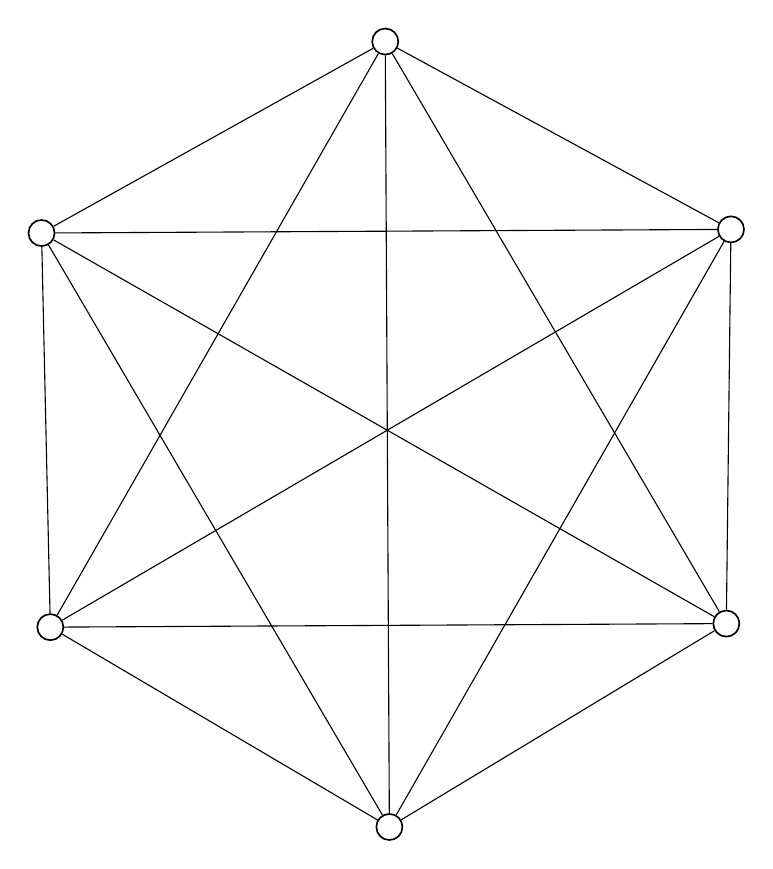
\begin{tikzpicture}[>={Latex},
  default/.style={draw=black, semithick, solid, fill=white, solid},
  every loop/.style={looseness=16}]
\node[default, circle] (A) at (-4.391002, 2.505132) {};
\node[default, circle] (B) at (-4.279503, -2.500332) {};
\node[default, circle] (C) at (0.026609, -5.038058) {};
\node[default, circle] (D) at (-0.026069, 4.936787) {};
\node[default, circle] (E) at (4.305587, -2.454942) {};
\node[default, circle] (F) at (4.364378, 2.551413) {};
\draw [] (A) -- (B) ;
\draw [] (A) -- (C) ;
\draw [] (A) -- (D) ;
\draw [] (A) -- (E) ;
\draw [] (A) -- (F) ;
\draw [] (B) -- (C) ;
\draw [] (B) -- (D) ;
\draw [] (B) -- (E) ;
\draw [] (B) -- (F) ;
\draw [] (C) -- (D) ;
\draw [] (C) -- (E) ;
\draw [] (C) -- (F) ;
\draw [] (D) -- (E) ;
\draw [] (D) -- (F) ;
\draw [] (E) -- (F) ;
\end{tikzpicture}
\end{document}
